\documentclass{standalone}
\usepackage{tikz}
\usepackage{gensymb}
\usetikzlibrary{decorations.footprints}

\tikzset{every picture/.style={line width=0.75pt}} %set default line width to 0.75pt

%molt cutre. Necessito treballar alguna cosa com:
%https://tex.stackexchange.com/questions/374338/geometric-inversion-of-an-image-png-jpg-bmp

\begin{document}

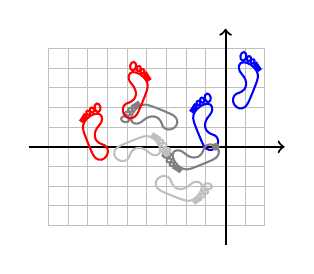
\begin{tikzpicture}[scale = 0.25,decoration={footprints,foot length=20pt}]
   
    \draw [step=1.0,lightgray,thin] (-9,-4) grid (2,5);
    \draw [->](-10,0) -- (3,0); %x-axis
    \draw [->](0,-5) -- (0,6); %y-axis
    \draw [decorate,blue] (0,0) -- (0,5);

    %faig rotació de taló esquerra
    \draw[decorate,gray,rotate around={90:(-0.5,0)}] (0,0) -- (0,5);
    \filldraw [gray] (-0.5,0) circle (4pt);

    %faig rotació contrària de punta esquerra
    \draw[decorate,lightgray,rotate around={-180:(-3,-0.3)}] (-0.5,0.5) -- (-5.5,0.5);
    \filldraw [lightgray] (-3,-0.3) circle (4pt);

    %faig rotació de taló esquerra
    \draw [decorate,red] (-5.6,-0.5) -- (-5.6,5);


\end{tikzpicture}

\end{document}
